
\section{Protocol Design}
Unlike the video bit-rate adaptation of FOV-aware streaming, Dante, from the perspective of reliability scheme, preferentially provisions the tiles, which are viewed by user with higher probability and are more important to user's QoE, with more FEC redundancy.  

%We consider the expected video quality loss caused by transmission loss and decoding dependencies of video codec, both of which depend on the FEC parameter adjusting procedure.	

\subsection{FEC Redundancy Adaptive Adjusting}
The aim of FEC adaptation is to find the optimal FEC redundancy for different regions in different frames. Above all, it is necessary to judge whether a kind of FEC redundancy is optimal. Obviously, the optimal FEC redundancy is obtained when the best video quality is achieved. Generally, PSNR is used to evaluate the video quality which is calculated via Mean Squared Error (MSE). So, we measure video quality or video distortion using MSE.


\subsubsection{optimization problem}

We consider that the optimal FEC redundancy is obtained if minimization of the video distortion, MSE, is achieved.
Given the tiles viewing probability distribution \cite{360ProbDASH}, estimated packet loss rate $\Pi _m^\alpha$, the optimal FEC redundancy for each layer of all frames can be obtained by solving the following optimization problem, which can be formalated as:
\begin{eqnarray}
&{\{ R_m^a\} _{1 \le m \le M,a \in Q}} = \arg \min (\sum\limits_{i = 1}^M {d_{m,effective}}).  \\
&{\rm{subject}}{~~\rm{to}}{~~~T^{tran}} \le {T_{GOP}}~~~~~~~~~~~~~~~~~, \\
&{\rm{and}}{~~~~~~\lambda ^p}(\Phi ) \le {\mu _p}\begin{array}{*{20}{c}}
{}
\end{array}{\rm{}},{\rm{}}~~~~~~~1 \le p \le P~~~,\\
&\begin{array}{*{20}{c}}
{{T^{tran}}{\rm{ = }}}&{\frac{{\sum\nolimits_{m = 1}^M {\sum\nolimits_{\alpha  \in Q} {(V_m^\alpha  \cdot (1 + R_m^a))} } }}{{t{r^{TFRC}}}}}
\end{array},\\
&{\lambda ^p}(\Phi ) = \lambda \frac{{\sum\nolimits_{m = 1}^M {\sum\nolimits_{\alpha  \in Q} {{{(V_m^\alpha  \cdot (1 + R_m^a))}_{_{\left\{ {\Phi _m^\alpha  \in p} \right\}}}}} } }}{{\sum\nolimits_{m = 1}^M {\sum\nolimits_{\alpha  \in Q} {V_m^\alpha } } }}.
\end{eqnarray}

Where, the minimization of the sum of video distortion for a GOP is the objective function, subject to constraints of both deadline and available bandwidth. And the decision variable, $\{ R_m^\alpha \}$, denotes the redundancy of the $\alpha$ layer for the m-th frame. The first constraint (Eq. (3)) indicates that, due to video's timeliness, the data of every GOP should be transmit to the client side before the delay constraint $T_{GOP}$.
Menwhile, ${V_m^\alpha }$ denotes the size of the $\alpha$ layer for the m-th frame. Given the packet size, S, the estimated round trip time, RTT and estimated packet loss rate, $\Pi_m^\alpha$, the tranmission time of GOP can be calculated by this procedure that the size of GOP, already considering the introduction of FEC redundancy, is divided by the transmission rate, $t{r^{TFRC}}$, according to \cite{TRFC}. 
The second constraint, (Eq. (4)), represent the video traffic rate, considering the introduction of FEC redundancy, is supposed to be not greater than the sum of available bandwidth of all paths.

$\Phi$, a vector, denotes the result of packet scheduling in the scheme of \cite{MPMTP}, which is composed of $\Phi
_m^\alpha {\rm{\{ }}\alpha  \in Q,1 \le m \le M{\rm{\} }}$,  imposed on the $\alpha$ layer for the m-th frame. And the value range of each $\Phi _m^\alpha $ is the serial number of available paths, like 0 to 1.








\subsubsection{The Analysis of Objective Function}

%So, we design a distortion-driven FOV-aware FEC adaptation.
The distortion computing model of the objective function is supposed to manifest the effect which FEC redundancy has on different regions.
By comparing the estimated expected value of video distortion after all kind of FEC redundancy provisioning, we can get the optimal FEC redundancy, corresponding to the optimal expected value of distortion. 

According to \cite{distortion_model} and \cite{CMT-VR}, 
The distortion of the m-th frame for every video GOP (group of pictures) can be formulated as:${d_m} = d_{m,trunc}(R_m,\pi) + {d_{m,drift}}$.
However, unlike non-360-degree videos, only a small portion of 360-degree videos spatially is perceived by users anytime. Furthermore, according to 360ProbDASH\cite{360ProbDASH}, each tile of 360-degree videos requested by users, is expected to be watched by users with a probability following Gaussian Distribution at any time. So we customize the traditional distortion model into the expected value of distortion, called as the effective distortion, which can be calculated in this schemes in which the distortion of each region is multiplied by its probability of viewing. 
As a result, for each video frame, the effective distortion is formulated as:
\[{d_{m,effective}} = \sum\limits_{\alpha  \in Q} {{\gamma ^\alpha }(d_{_{m,trunc}}^{^\alpha } + d_{_{m,drift}}^{^\alpha })}\]
where Q denotes the layer set of 360-degree videos, which includes FOV layer, cushion layer and outmost layer, as depicted in Figure 3. And given $\alpha $
layer, ${\gamma ^\alpha }$ denotes the accumulated viewing probability, formulated as:
\begin{equation}
{\gamma ^\alpha } = \sum\limits_{i = 1}^{{\Omega ^\alpha }} {{p_i} \cdot
	{S_i}}
\end{equation}
Where ${p_i}$ stands for viewing probability of the i-th tile in the $\alpha $
layer, ${S_i}$ denotes area of the i-th tile and
${\Omega ^\alpha }$ denotes tiles set of the corresponding layer. 

Obvious, the tiles of FOV, requested by users and viewed by users with higher probabilities, are attached with greater weights than non-FOV. Thus, improving the distortion of the FOV region can bring more performance gain in video distortion than non-FOV region. 

Meanwhile, given the estimated packet loss rate $\pi _{m,\alpha }^t$,  $d_{m,trunc}^\alpha$, denotes the expected value of MSE with regard to FEC redundancy provisioning for the $\alpha$ layer of the m-th frame, which is
formulated as:
\[d_{m,trunc}^\alpha (\pi _{m,\alpha }^t) = \widehat \delta _m^\alpha  + \Pi _m^\alpha (\pi _{m,\alpha }^t)\cdot\delta _m^\alpha ,1 \le m \le M\]	

where, $d_{m,trunc}^\alpha$ is proportional to $\Pi _m^\alpha$. And given a frame $m$, region $\alpha$, FEC-redundancy rate $k$, and estimated packet loss rate $\pi _{m,\alpha }^t$,
$\Pi _m^\alpha$ denotes the percentage of lost symbols for the $\alpha$ layer of the m-th frame, which is
formulated as ,
\begin{eqnarray}
&\Pi _m^\alpha (\pi _{m,\alpha }^t) = \left\{ {\begin{array}{*{20}{l}}
{0,\begin{array}{*{20}{c}}
{}
\end{array}if\begin{array}{*{20}{c}}
{\pi _{m,\alpha }^t + (1 - \pi _{m,\alpha }^t)}
\end{array}\cdot\pi _{m,\alpha }^o < \frac{{n - k}}{n},}\\
{\begin{array}{*{20}{c}}
{\pi _{m,\alpha }^t + (1 - \pi _{m,\alpha }^t)}
\end{array} \cdot \pi _{m,\alpha }^o,\begin{array}{*{20}{c}}
{}
\end{array}{\rm{otherwise}}.}
\end{array}} \right.
\end{eqnarray}

where given the $\alpha$ layer of the m-th frames $(n-k)$, denotes the number of FEC repair packets, and $\frac{{n - k}}{n}$ stands for tolerant packet loss rate and $\pi _{m,\alpha }^o$ denotes the overdue loss rate. Obviously, $\Pi _m^\alpha$ is equal to 0 if the provisioning of redundant repair packets is sufficient for countering packet drops caused by transmission loss and expired arrival. 



\subsubsection{An Algorithm To Solve The Optimal Problem}
According to (Eq. 7), the 



We, first determine the total number of FEC repair packets for a GOP, according to (Eq
Essentially, the optimal problem is a discrete optimization problem. Meanwhile, it's impractical to derive the optimal solution with polynomial time complexity, and the greedy search is not applicable for real time applications. To solve this problem, we design a fast research algorithm, which complexity is $O(N \cdot M \cdot Q)$, to obtain a sub-optimal solution of FEC redundancy adaptive problem, shown in Algorithm 1. 

\begin{algorithm}[!h] 
	\scriptsize
	\centering 
	\caption{FEC redundancy adaptative algorithm}%算法标题      
	\begin{algorithmic}[1]%一行一个标行号
		\STATE $R = \min (Eq.~(3), Eq.~(4))$ , according to delay constraints, Eq. (3) and
		bandwidth constraints Eq. (4),
		\FOR{$\alpha  \in Q$}  
		
		\STATE Calculate $\gamma ^\alpha$ , according to Eq. (1),
		
		\ENDFOR
		
		\STATE $N = \frac{V}{S} \cdot (1+R)$ 
		
		\FOR{$i = 1{\rm{ }} to {\rm{ }}N$}
		\STATE $index{\rm{ }} = {\rm{ }}0,{\rm{ }}{\Delta _d}{\rm{ }} = 0$
		\FOR{$m = 1{\rm{ }}to{\rm{ }}M$}
		\FOR{$\alpha  \in Q$}
		
		\STATE ${d_{effective}} = \sum\limits_{0 \le m \le M} {\sum\limits_{\alpha 
				\in Q} {{\gamma ^\alpha }(d_{_{m,trunc}}^{^\alpha } + d_{_{m,drift}}^{^\alpha
				})} } $
		\STATE ${N_{m,\alpha }} = {N_{m,\alpha }} + 1$
		\STATE $\Delta  = \left| { - {d_{effective}} + \sum\limits_{0 \le m \le M}
			{\sum\limits_{\alpha  \in Q} {{\gamma ^\alpha }(d_{_{m,trunc}}^{^\alpha } +
					d_{_{m,drift}}^{^\alpha })} } } \right|$
		\STATE ${N_{m,\alpha }} = {N_{m,\alpha }} - 1$
		\IF{$\Delta  \ge {\Delta _d}{\rm{ }}$}
		\STATE $index{\rm{ }} = m,\begin{array}{*{20}{c}}
		{layer}
		\end{array} = \alpha ,{\Delta _d} = \Delta$
		\ENDIF
		\ENDFOR 
		\ENDFOR
		\STATE ${N_{index, layer }} = {N_{index, layer }} + 1$
		\ENDFOR
		\RETURN${\left\{ {{R_{m,\alpha }} = \frac{{{N_{m,\alpha }}{\rm{ - }}{K_{m,\alpha }}}}{{{K_{m,\alpha }}}}} \right\}_{(1 \le m \le M,\alpha  \in Q)}}$
	\end{algorithmic}  
\end{algorithm} 




\subsection{System Overview}

Dante is proposed to support high-quality 360-degree video
streaming service over the wireless network. In Dante, UDP combined with the systematic FEC, RS code, is integrated to provide data delivery service over wireless networks. And only the data of I frames is retransmitted if no ACK is received by the server in time ${T^I}$, in order to guarantee the video data received is decodable by video codec.
Besides, TCP is supplementary to exchange control information, which is of significance. The overall protocol architecture is illustrated in Figure 2.

\begin{figure*}[ht]
	\centering
	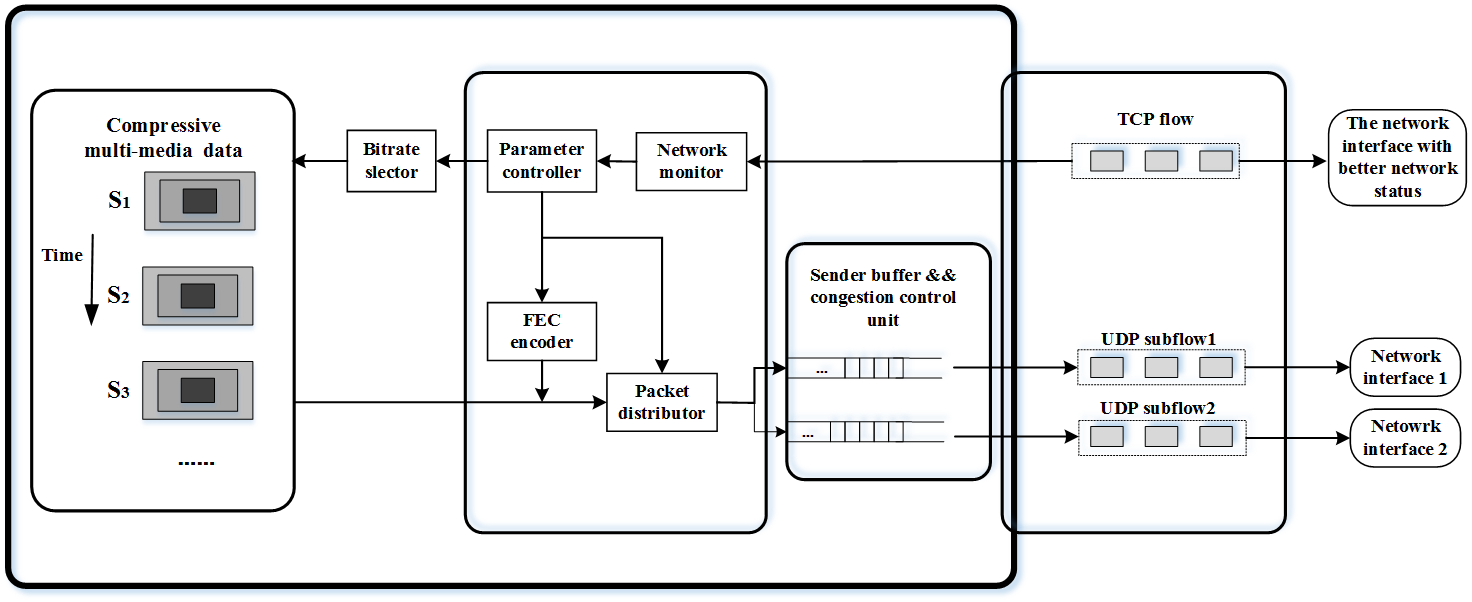
\includegraphics[scale=0.4]{paper_figs/architecture_V2.png}
	\caption{The Architecture of Protocol}
	\label{paper_figs:pathdemo}
\end{figure*}
